\chapter{追加実験}

第4章での考察を踏まえTravelatARの改良,実験環境の改善をし,追加実験を行った.

\section{TravelatARの改良}
第4章での考察を踏まえて行ったTravelatARの改良について示す.
バーチャル床の使用を以下の通り変更した.
「目の前で床が消えるので,そこで現実に戻されているような気がする」
とあったことから,バーチャル床を消すタイミングが速いことを確認できたため,
ユーザが踏んだ際では無く通り過ぎた際に消えるよう設定の変更した.
また,バーチャル床の動かし方は,従来の動き方の「前からユーザに向かってくる」と新しく「後ろからユーザを追い越す」\figref{fig:14}
の2つの動かし方をする.
\begin{figure}[H]
    \centering
    \fbox{
        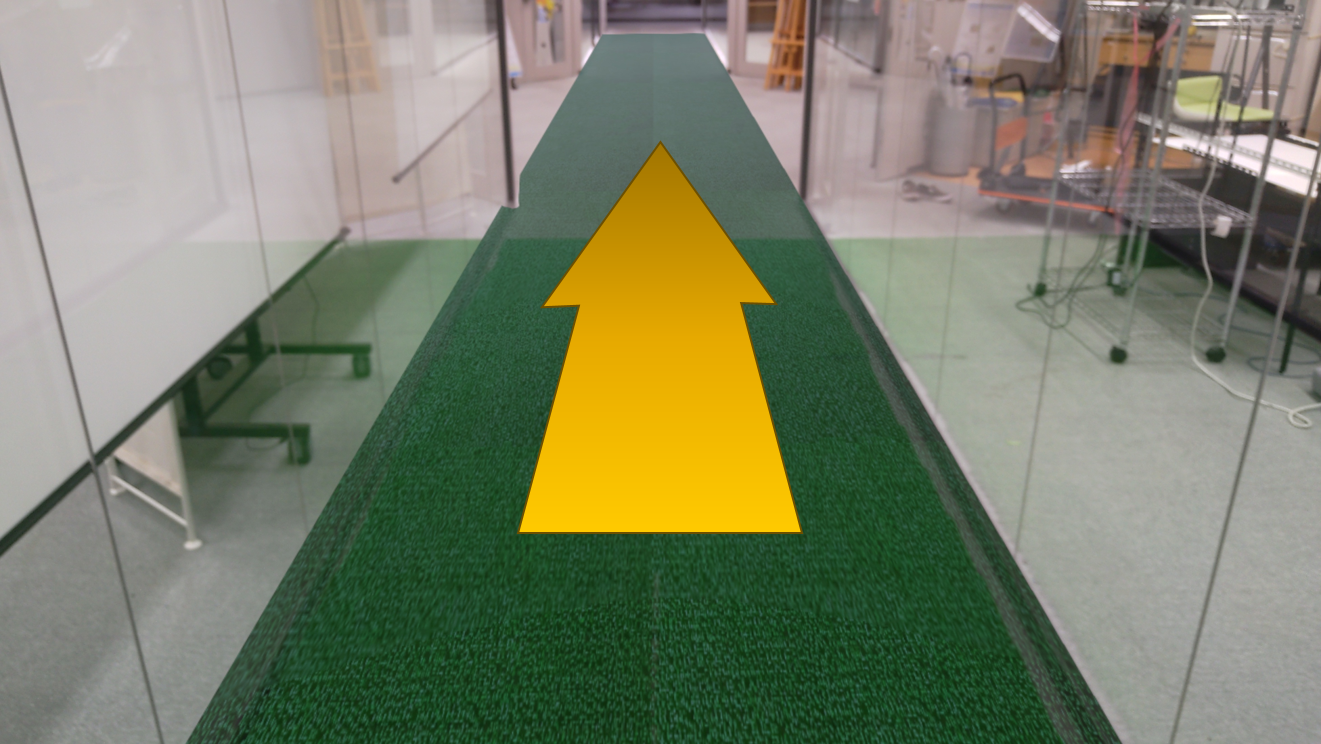
\includegraphics[width=0.7\linewidth]{fig/14.png}
    }
    \caption{後ろからユーザを追い越すバーチャル床のイメージ}
    \label{fig:14}
\end{figure}

\section{実験環境}
被験者は20代の男性7名である.
実験環境を\figref{fig:addgaiyo}に示す.
被験者に付けていたiPhone11 proは付けず,
歩いてもらうコース上には通過センサーとArduino\figref{fig:13.1}を\figref{fig:13}のよう設置する\cite{tuka}.
これにより,正確なユーザの歩行速度を測った.
また,\figref{fig:siten2}コースの照明を消すことで「表示されている床に透明感が強く,実際の床が見え,あまり影響がないように感じた」
「芝が虹色になっている部分がありました」といった照明によるテクスチャの評価への影響を軽減させた.

\begin{figure}[H]
    \centering
    \fbox{
        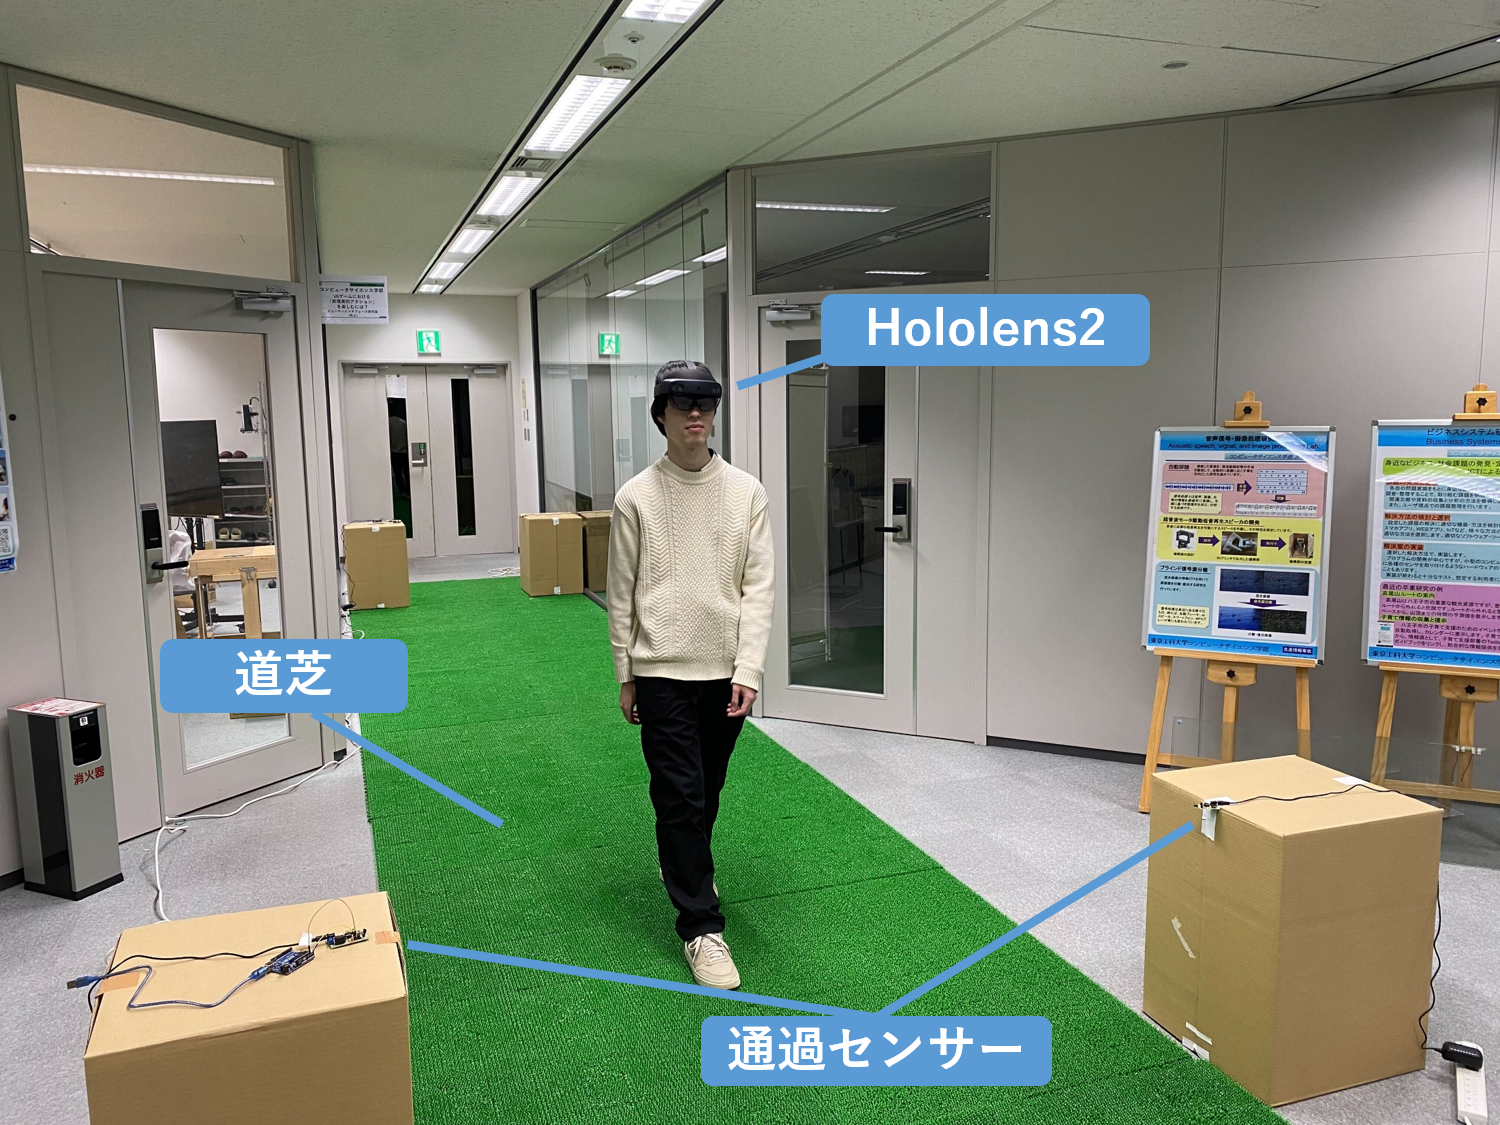
\includegraphics[width=0.7\linewidth]{fig/gaiyo.png}
    }
    \caption{追加実験での実験環境}
    \label{fig:addgaiyo}
\end{figure}
\begin{figure}[H]
    \centering
    \fbox{
        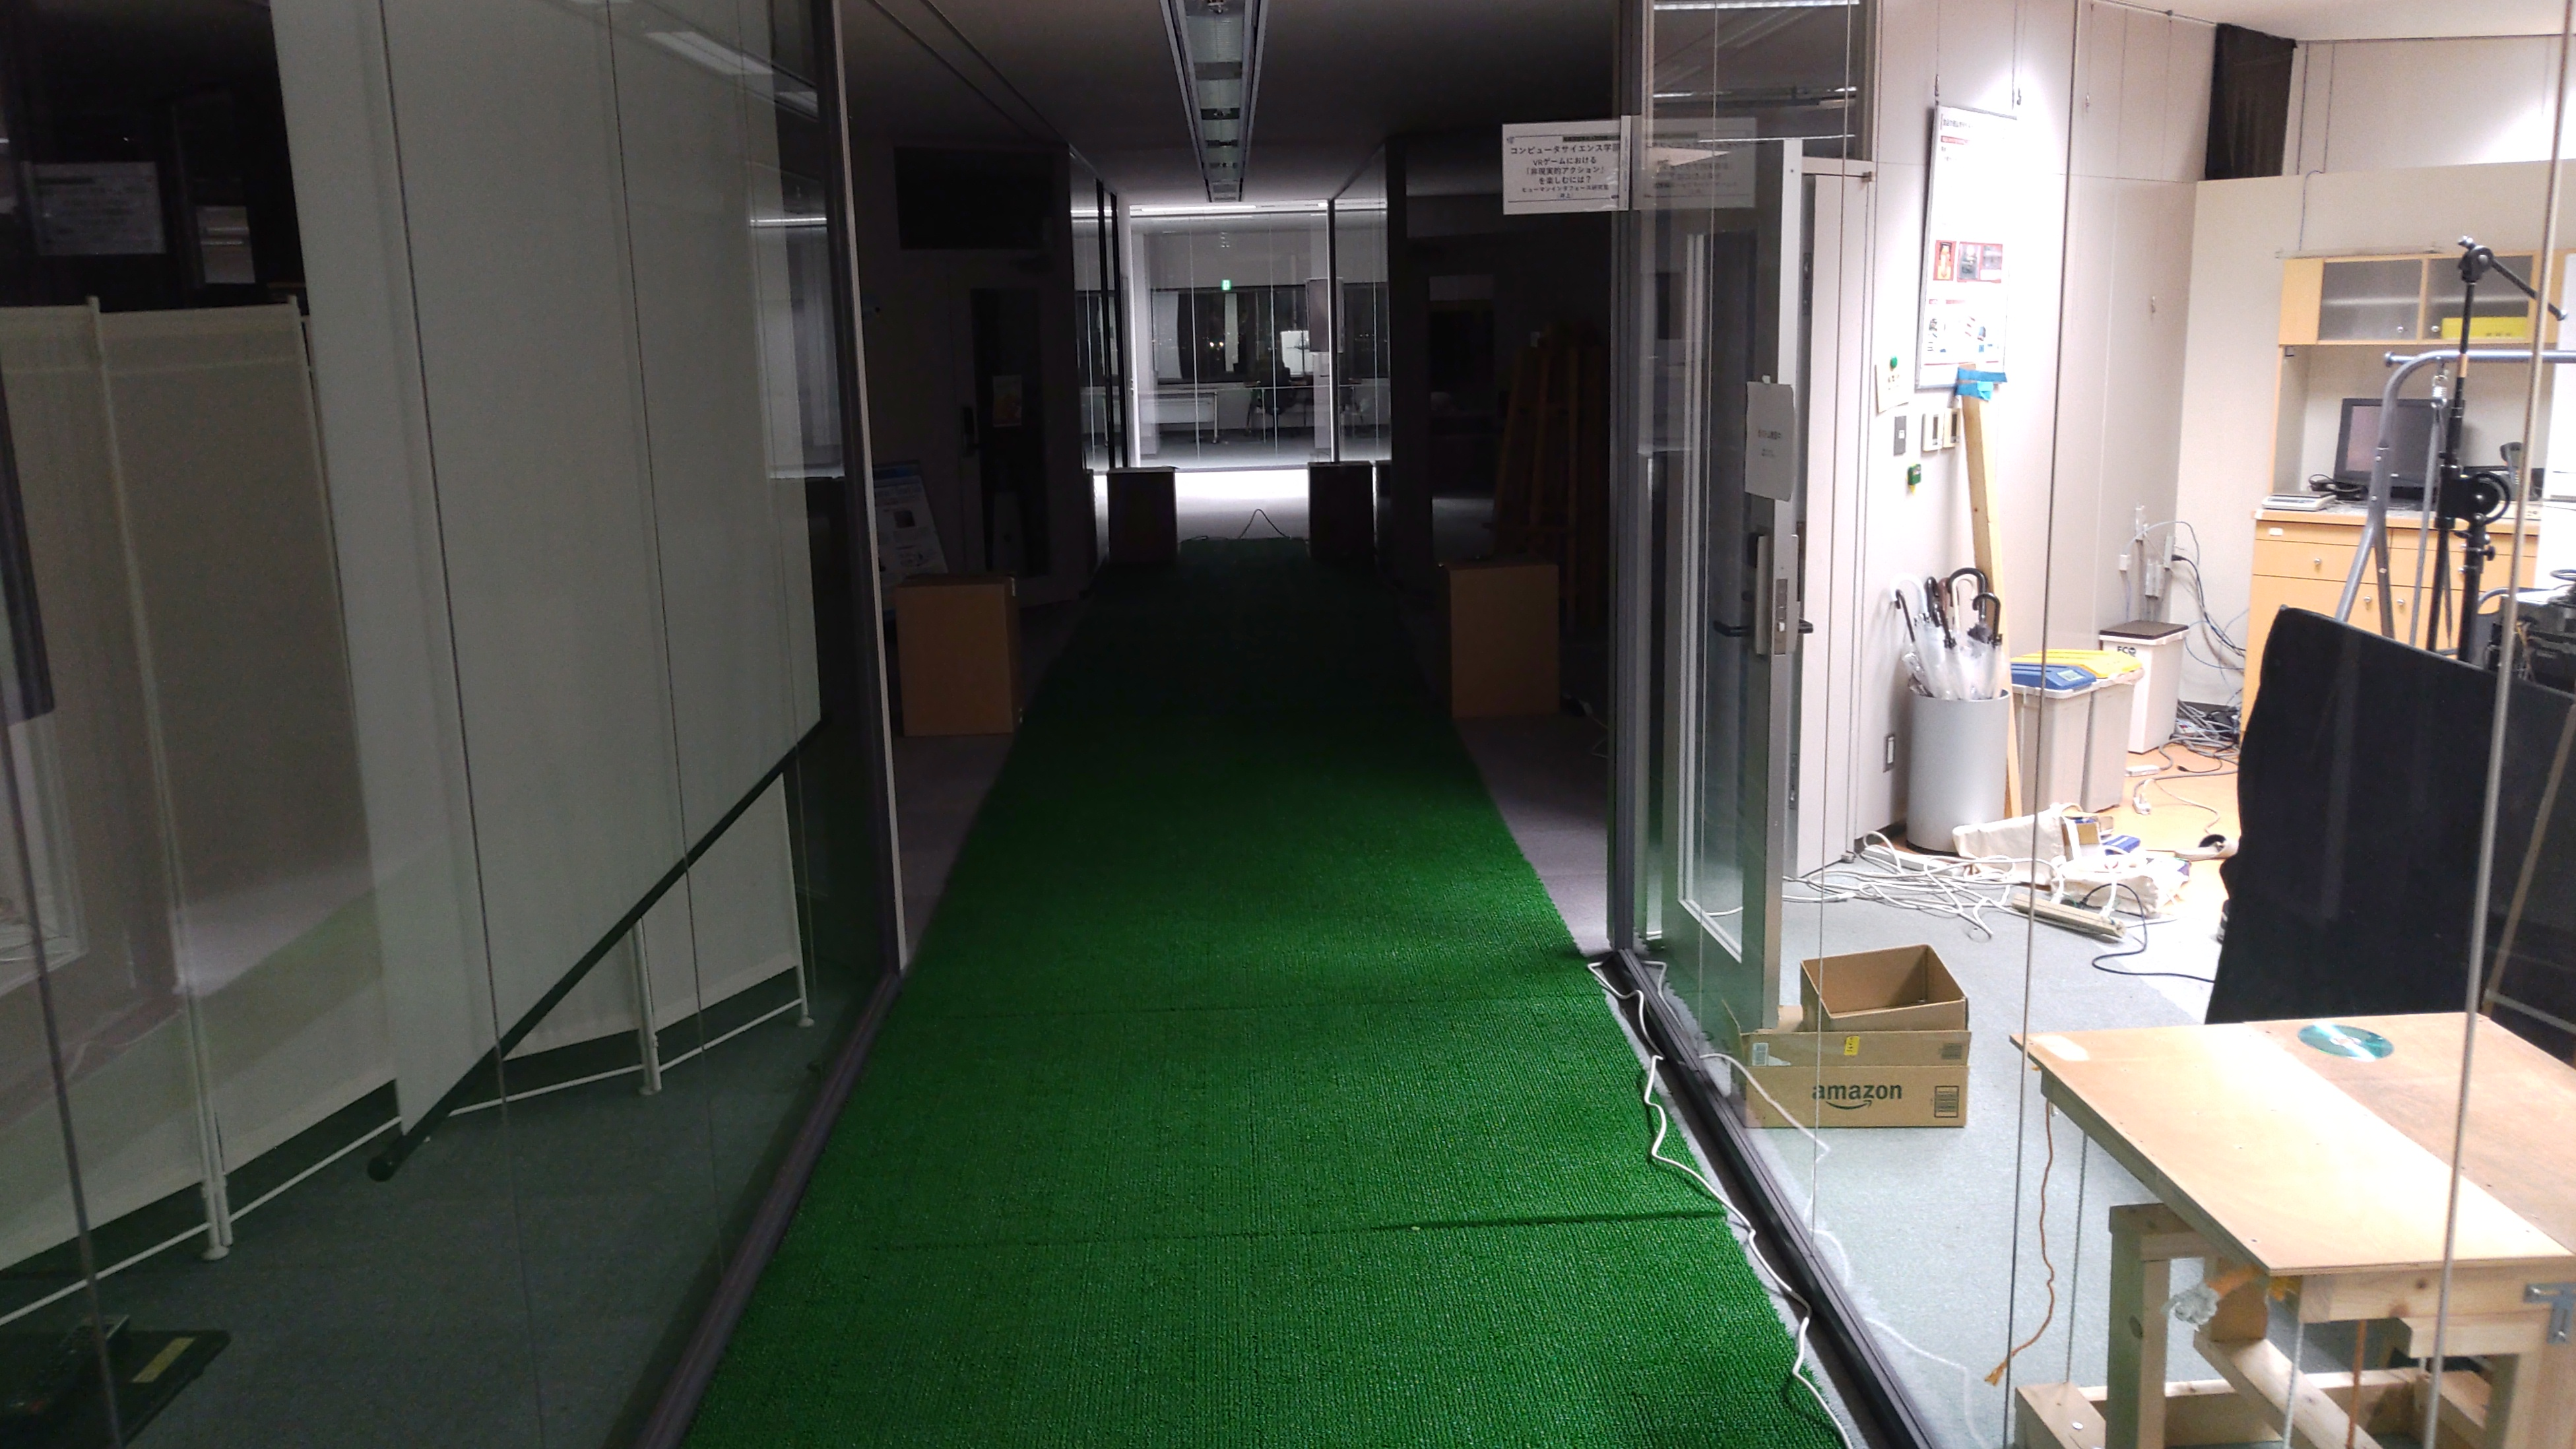
\includegraphics[width=0.7\linewidth]{fig/siten2.jpg}
    }
    \caption{実際に照明を消した実験環境}
    \label{fig:siten2}
\end{figure}

\begin{figure}[H]
    \centering
    \fbox{
        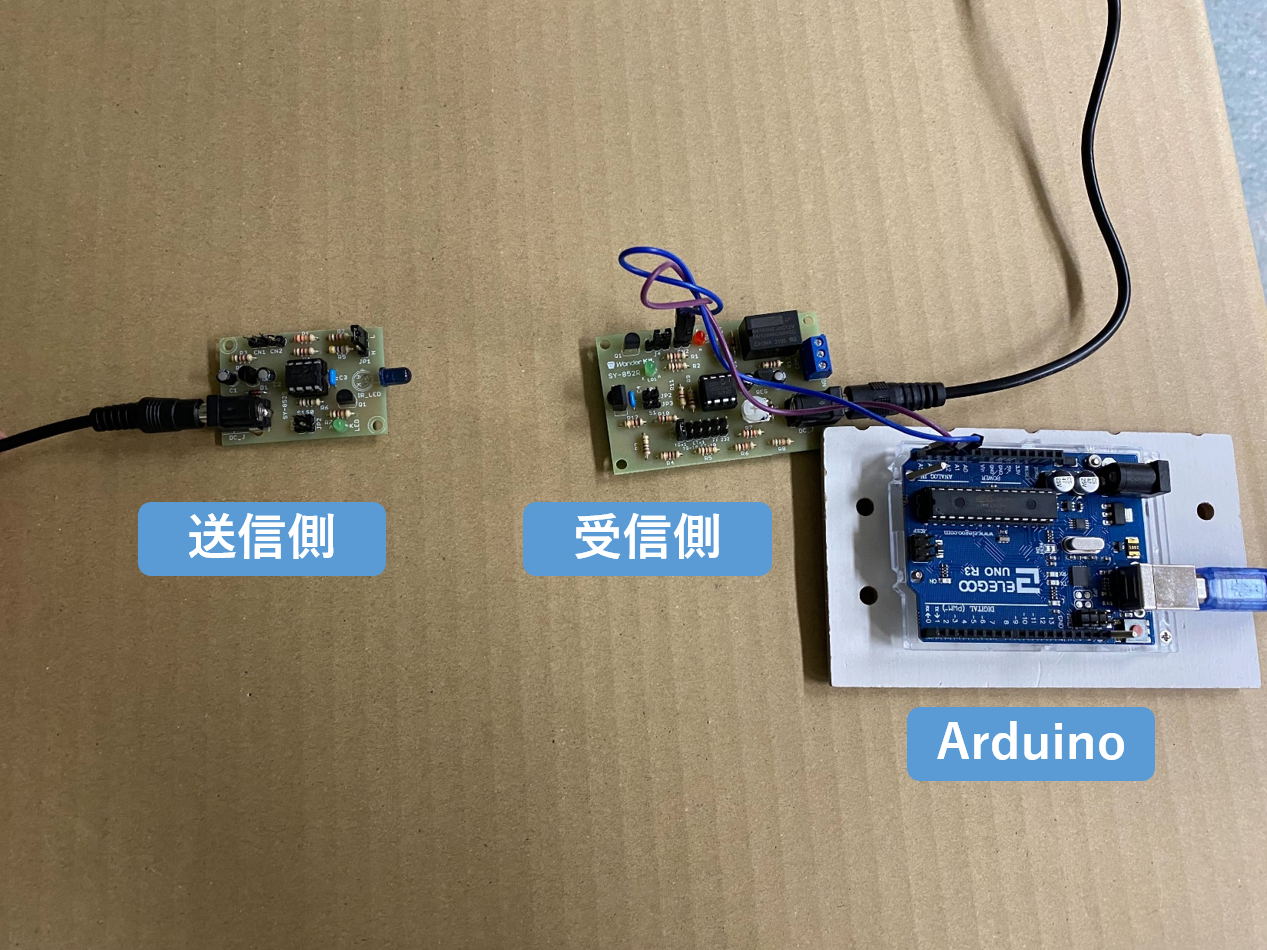
\includegraphics[width=0.7\linewidth]{fig/sensor.png}
    }
    \caption{通過センサーとArduino}
    \label{fig:13.1}
\end{figure}

\begin{figure}[H]
    \centering
    \fbox{
        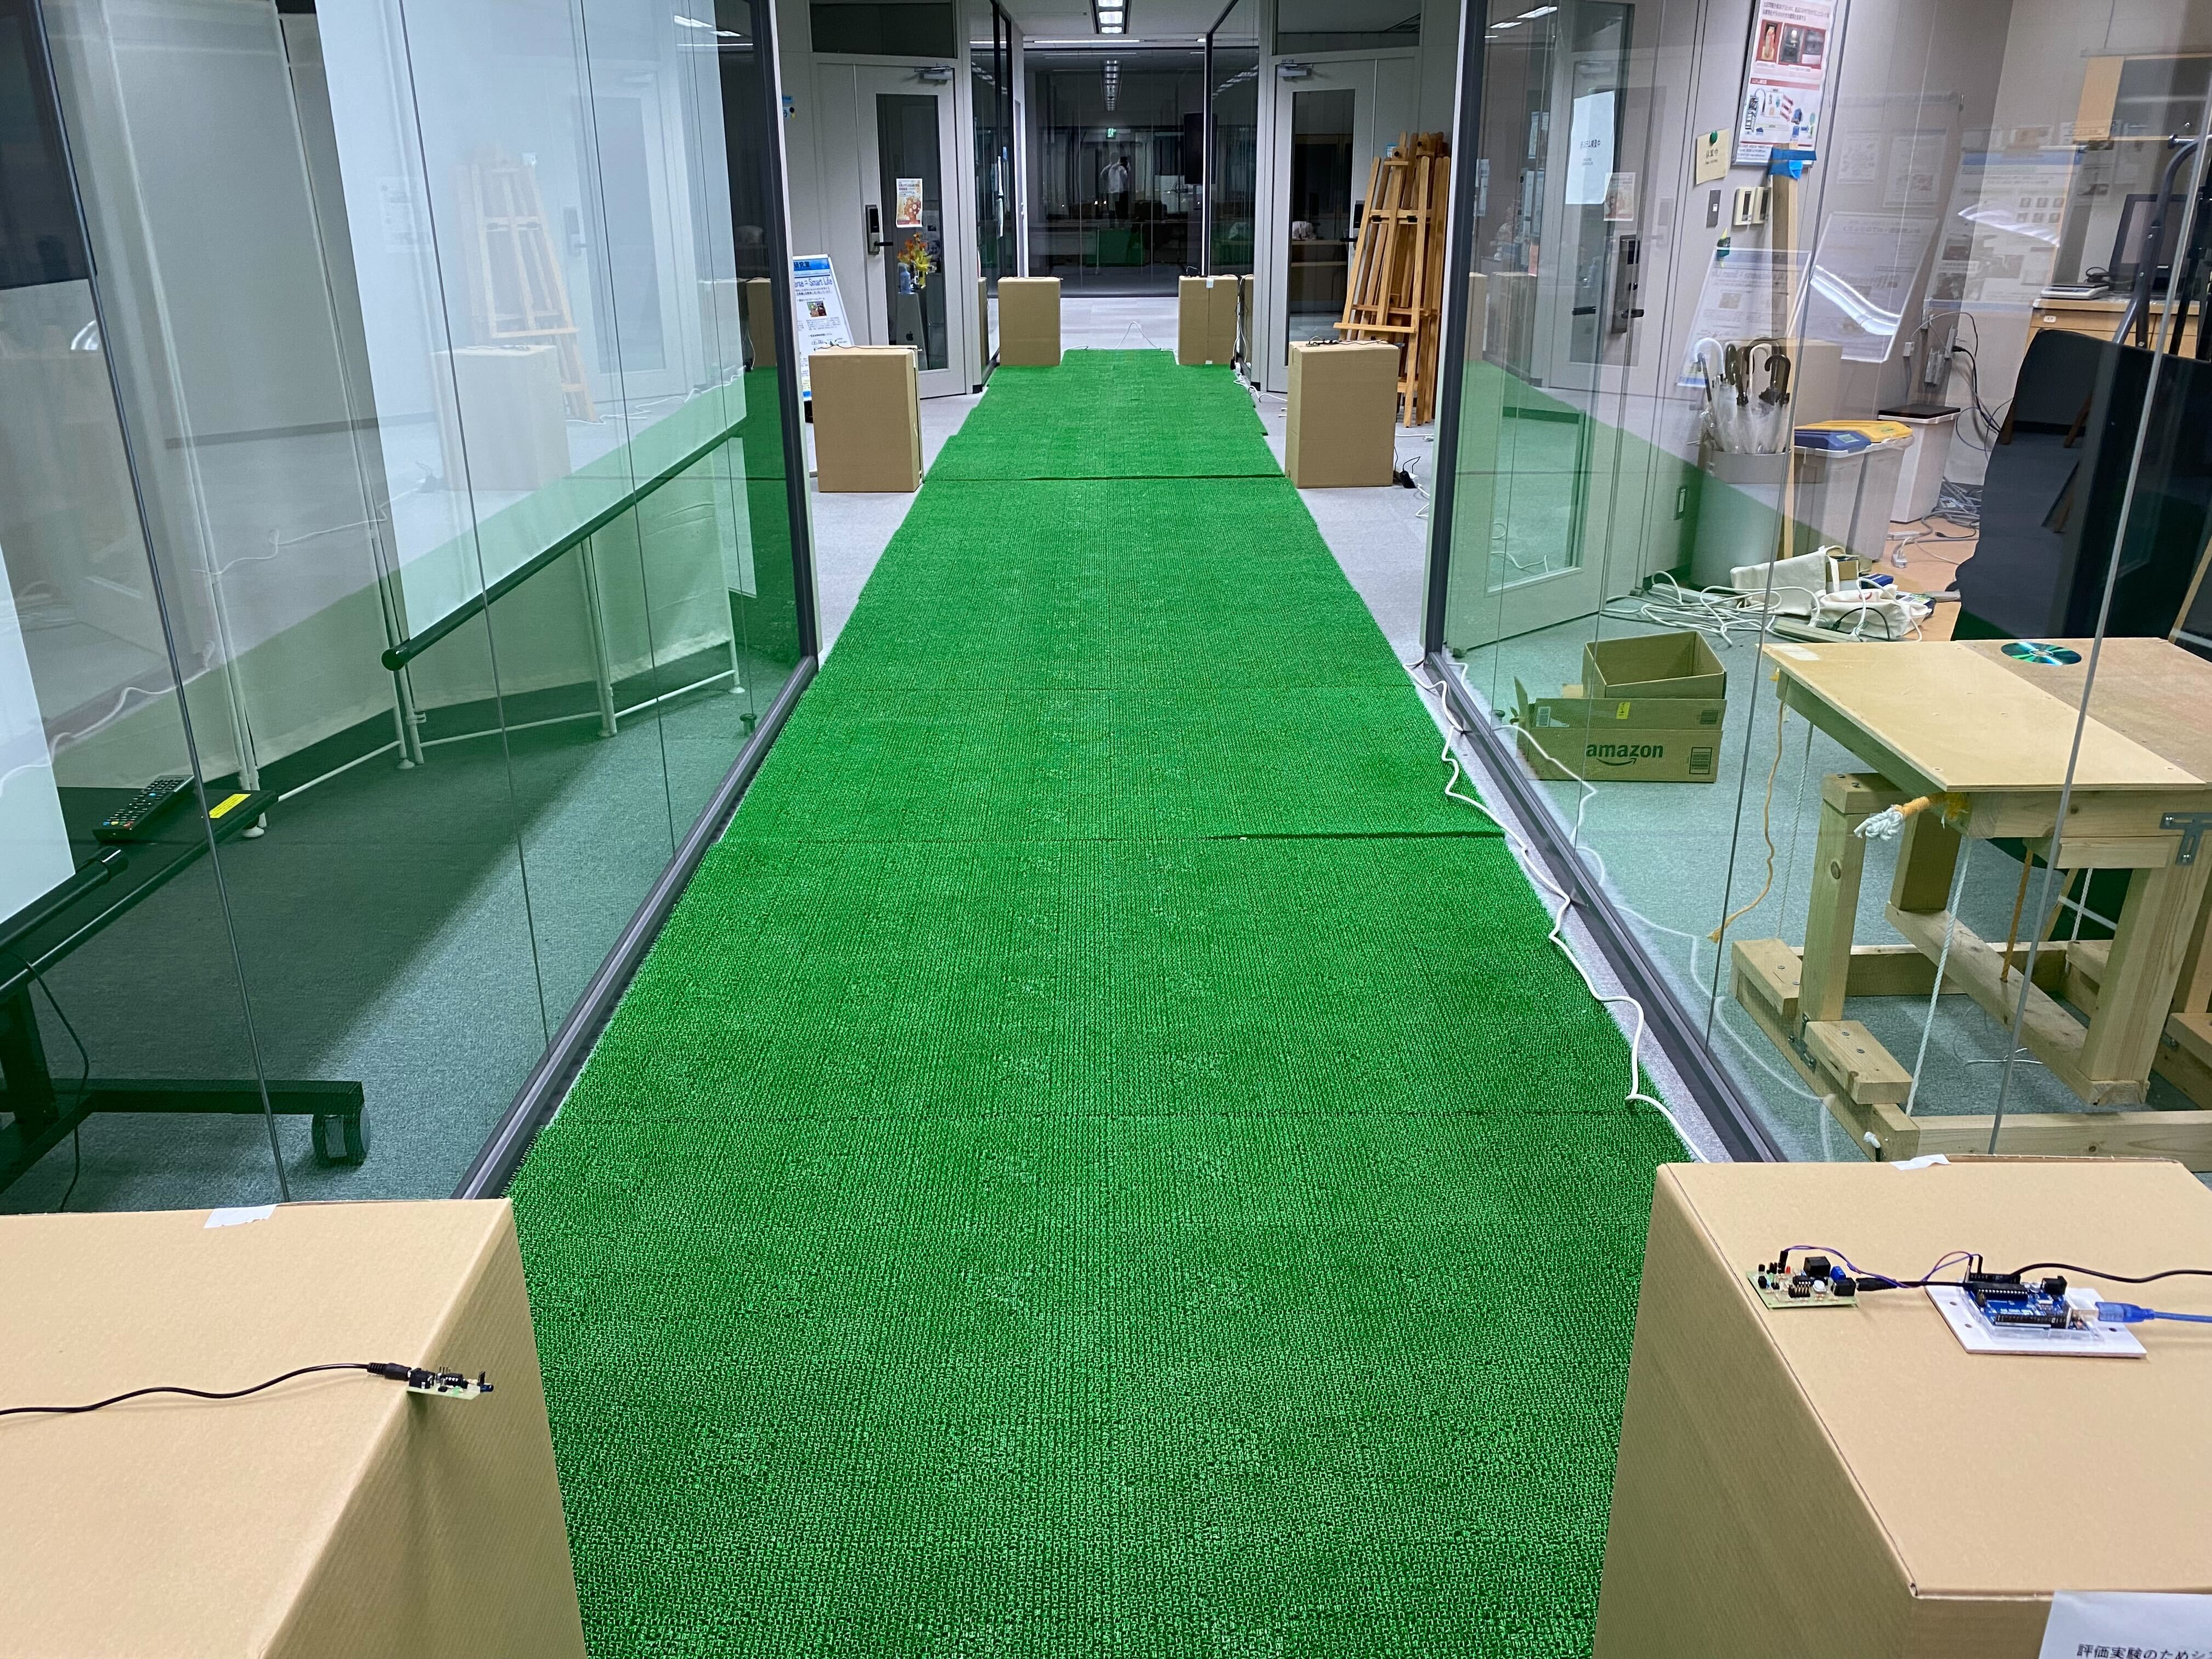
\includegraphics[width=0.7\linewidth]{fig/13.jpg}
    }
    \caption{通過センサーの配置}
    \label{fig:13}
\end{figure}



\section{実験手順}
実験手順を以下に示す.
\begin{enumerate}
    \item スタート地点に直立してもらった
    \item 指定距離歩いてもらった
    \item 歩き終わった位置で直立してもらった
\end{enumerate}
上記の手順を3回同じシステムで繰り返してもらい,それを1セットとした.
また,被験者は1セット終わるたびにアンケートを回答してもらうと共に休憩した.
この手順をシステムを使用していない状態のHoloLens2を装着した状態,
12種類のテクスチャと2種類のバーチャル床の動き方の計25セット行ってもらった.

\section{評価方法}
第4章での評価と同じく定性評価と定量評価を行う.


定性評価では,第4章でのアンケート項目に
前実験で「速く移動しているようにも感じるし,たくさん移動しているようにも感じた」というコメントがあったことから,
距離感に対しての影響の調査として
「システム未使用時に比べて歩行距離が短く感じたか」「システム未使用時に比べて歩行距離が長く感じたか」
をそれぞれ1(まったく感じなかった)~5(非常に感じた)までの5段階のリッカート尺度を用いた形で追加した.


定量評価では通過センサーを用いたタイマーから取得した時間で第4章と同じ評価方法をとる.
また,スタート地点とゴール地点の中間地点にもセンサーを置くことで中間地点での歩行時間を用いた評価も行う.
\section{実験結果}
定性評価の結果を以下に示す.
\figref{fig:f1}にシステム未使用時に比べ,バーチャル床が前から迫ってくることで速い速度感を得たか,
\figref{fig:f2}にシステム未使用時に比べ,バーチャル床が前から迫ってくることで遅い速度感を得たか
\figref{fig:f3}にシステム未使用時に比べ,バーチャル床が前から迫ってくることで歩行距離が短く感じたか,
\figref{fig:f4}にシステム未使用時に比べ,バーチャル床が前から迫ってくることで歩行距離が長く感じたか,
\figref{fig:b1}にシステム未使用時に比べ,バーチャル床が後ろから追い越してくることで速い速度感を得たか,
\figref{fig:b2}にシステム未使用時に比べ,バーチャル床が後ろから追い越してくることで遅い速度感を得たか,
\figref{fig:b3}にシステム未使用時に比べ,バーチャル床が後ろから追い越してくることで歩行距離が長く感じたか,
\figref{fig:b4}にシステム未使用時に比べ,バーチャル床が後ろから追い越してくることで歩行距離が短く感じたか,
\figref{fig:simi}にバーチャル床は本物の床が動いているように見えたかのアンケート結果を示す.
これらの棒グラフは,左から1(まったく感じなかった)~5(非常に感じた),円グラフでは1(まったく見えなかった)~5(非常に見えた)となっている.
バーチャル床が前から迫ってくる場合,
\figref{fig:f1},\figref{fig:f2}から,5YR天然のテクスチャ(\figref{fig:ff5yr})が一番速い速度感を与えることがわかり,バーチャル床が前から迫ってく表示の仕方をするとどのテクスチャも遅い速度感を与えないということが分かった.
\figref{fig:f3},\figref{fig:f4}から,体感歩行距離が短く感じることはどのテクスチャでもなかったが,5G天然(\figref{fig:fl5G})と5B砂利(\figref{fig:fl5B})は歩行距離を長く感じさせる効果があるとわかった.
バーチャル床が後ろから追い越してくる場合では,
\figref{fig:b1},\figref{fig:b2}から,バーチャル床が後ろから追い越してくることで,速い速度感は与えないことがわかった.しかし,5YR人工(\figref{fig:bs5YR})は遅い速度感を与えることがわかった.
また,\figref{fig:b3},\figref{fig:b4}から,ほとんどのテクスチャは体感歩行距離に影響を与えないことがわかった.
\figref{fig:simi}から,5RP天然(\figref{fig:c5RP})がもっとも本物の床が動いているように見えてということがわかった.
\begin{figure}[H]
    \centering
    \fbox{
        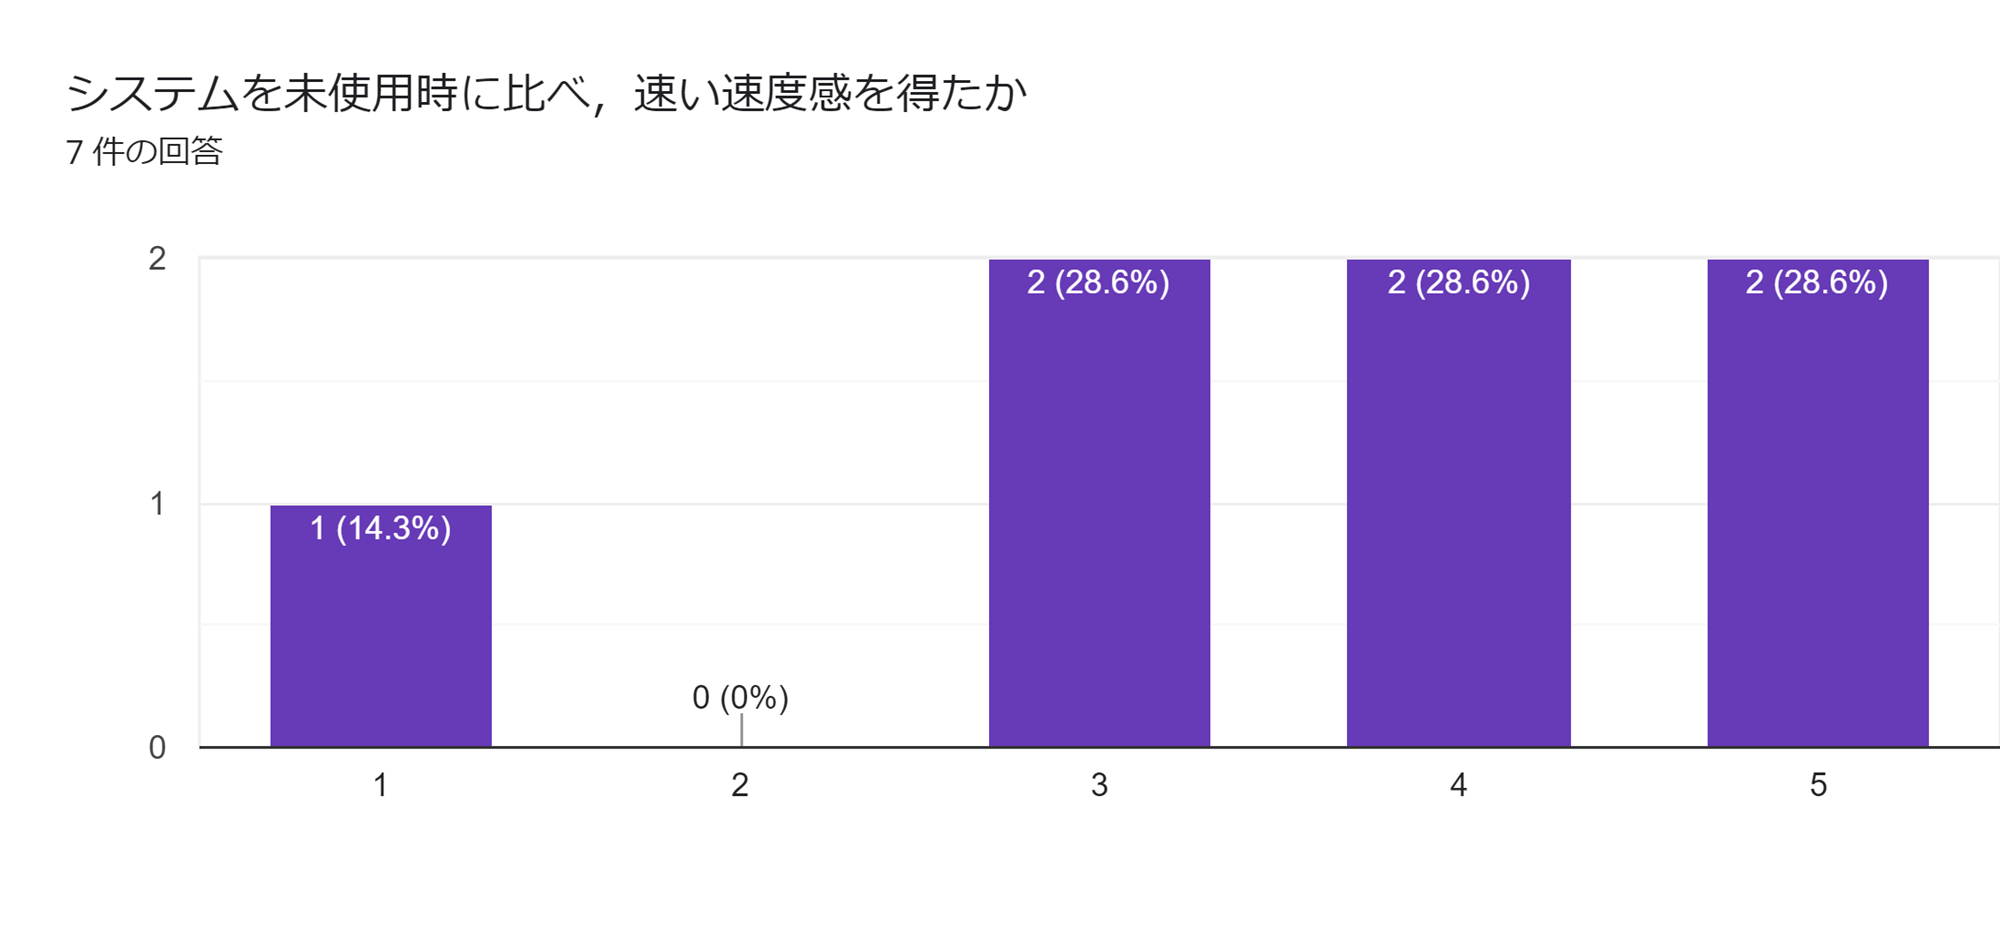
\includegraphics[width=0.8\linewidth]{fig/前早5YR天然.png}
    }
    \caption{システム未使用時に比べ,バーチャル床が前から迫ってくることで速い速度感を得たかの結果(5YR天然)}
    \label{fig:ff5yr}
\end{figure}
\begin{figure}[H]
    \centering
    \fbox{
        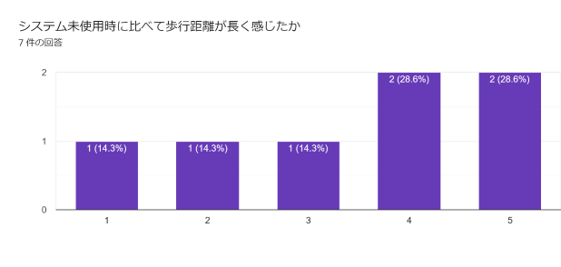
\includegraphics[width=0.8\linewidth]{fig/前長5G天然.png}
    }
    \caption{システム未使用時に比べ,バーチャル床が前から迫ってくることで歩行距離が長く感じたかの結果(5G天然)}
    \label{fig:fl5G}
\end{figure}

\begin{figure}[H]
    \centering
    \fbox{
        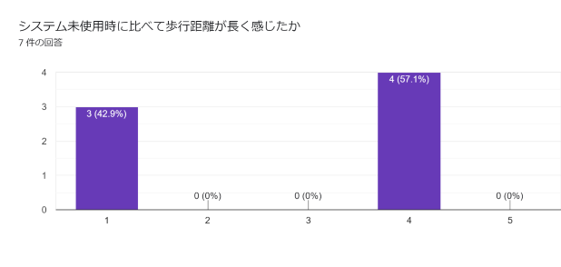
\includegraphics[width=0.8\linewidth]{fig/前長5B砂利.png}
    }
    \caption{システム未使用時に比べ,バーチャル床が前から迫ってくることで歩行距離が長く感じたかの結果(5B砂利)}
    \label{fig:fl5B}
\end{figure}

\begin{figure}[H]
    \centering
    \fbox{
        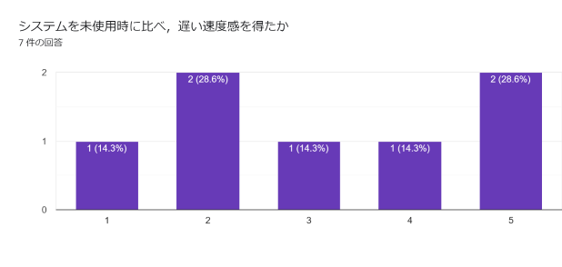
\includegraphics[width=0.8\linewidth]{fig/後遅5YR人工.png}
    }
    \caption{システム未使用時に比べ,バーチャル床が後ろから追い越してくることで遅い速度感を得たかの結果(5YR人工)}
    \label{fig:bs5YR}
\end{figure}

\begin{figure}[H]
    \centering
    \fbox{
        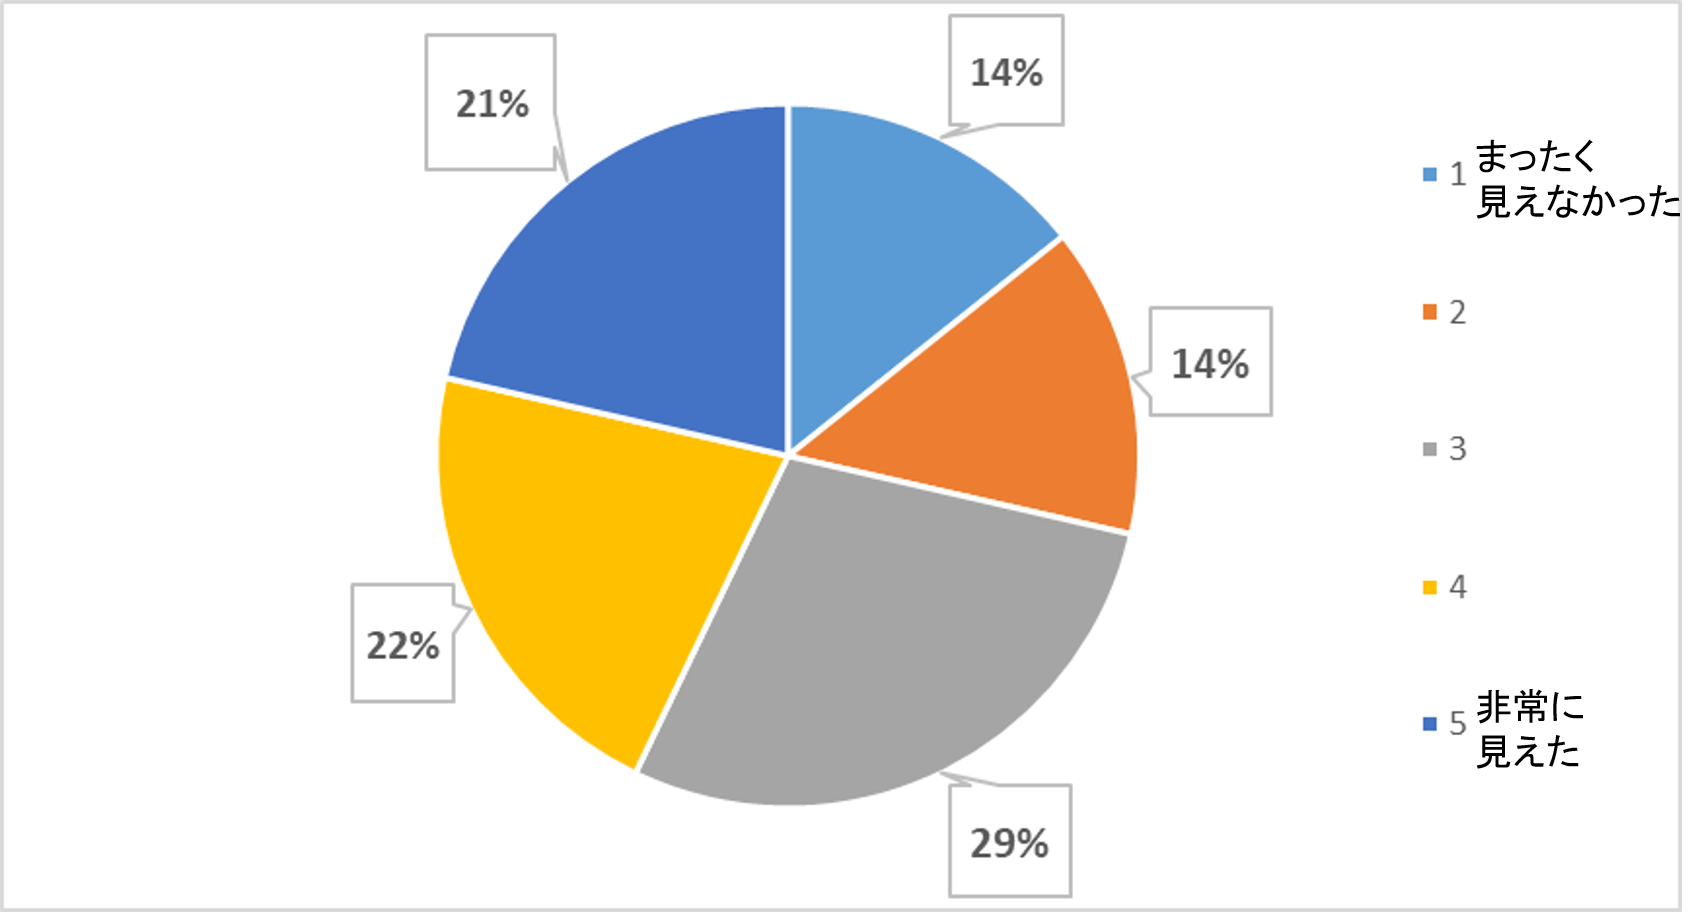
\includegraphics[width=0.8\linewidth]{fig/色5RP天然.png}
    }
    \caption{バーチャル床は本物の床が動いているように見えたかの結果(5RP天然)}
    \label{fig:c5RP}
\end{figure}

定量評価の結果を以下に示す.
\figref{fig:maehalf}にシステム未使用時とバーチャル床が前から迫ってくるシステム使用時の中間地点までの時間差の一覧,
\figref{fig:maetime}にシステム未使用時とバーチャル床が前から迫ってくるシステム使用時のゴールまでの時間差の一覧.
\figref{fig:usirohalf}にシステム未使用時とバーチャル床が後ろから追い越してくるシステム使用時の中間地点までの時間差一覧.
\figref{fig:usirotime}にシステム未使用時とバーチャル床が後ろから追い越してくるシステム使用時のゴールまでの時間差一覧を示す.
バーチャル床が前から迫ってくる場合,
\figref{fig:maehalf}から,中間地点では被験者によって時間の差はプラスマイナスが分かれたが
\figref{fig:maetime}から,5YR人工(\figref{fig:5YRjinko})とリアルテクスチャである5G人工(\figref{fig:5Gjinko})はゴールまでの歩行時間が長くなっていた.

バーチャル床が後ろから追い越してくる場合では,
\figref{fig:usirohalf}から,中間地点では被験者によって時間の差はプラスマイナスが分かれた.
しかし,\figref{fig:usirotime}から,5YR天然(\figref{fig:5YRten}),5RP天然(\figref{fig:5RPten}),5RP人工(\figref{fig:5RPjinko}),ではゴール時の全ユーザが歩行時間が短くなっていた.
これらの結果は,SSQによる映像酔いの調査結果からの影響は確認できなかった.
\begin{figure}[H]
    \centering
    \fbox{
        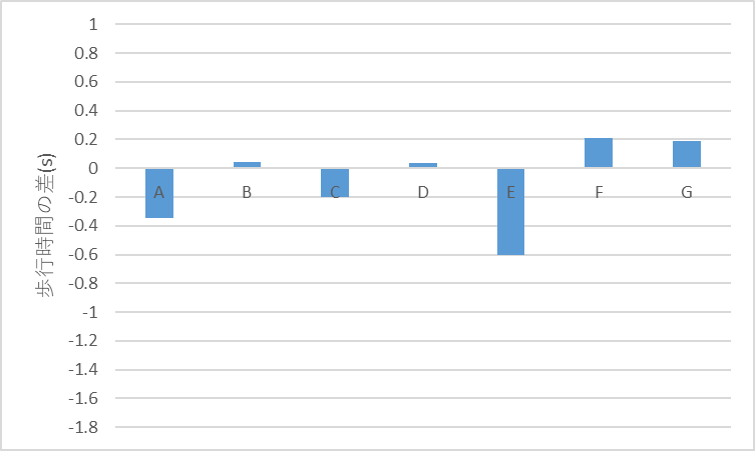
\includegraphics[width=0.8\linewidth]{fig/前速度早5YR人工.png}
    }
    \caption{システム未使用時とバーチャル床が前から迫ってくるシステム使用時のゴールまでの時間差(5YR人工)}
    \label{fig:5YRjinko}
\end{figure}

\begin{figure}[H]
    \centering
    \fbox{
        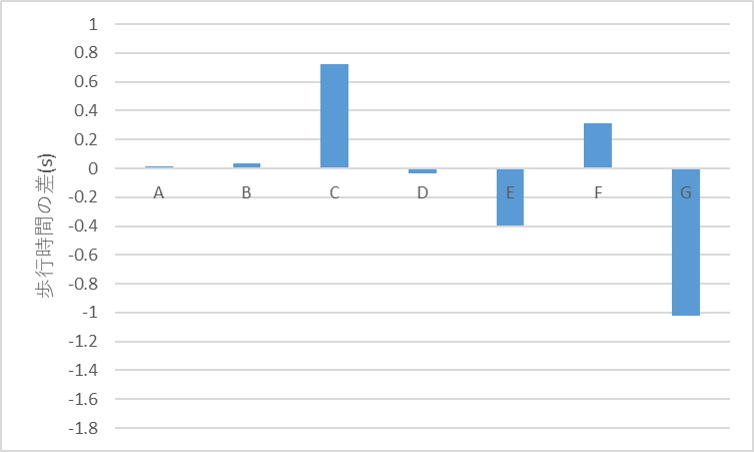
\includegraphics[width=0.8\linewidth]{fig/前速度早5G人工.png}
    }
    \caption{システム未使用時とバーチャル床が前から迫ってくるシステム使用時のゴールまでの時間差(5G人工)}
    \label{fig:5Gjinko}
\end{figure}

\begin{figure}[H]
    \centering
    \fbox{
        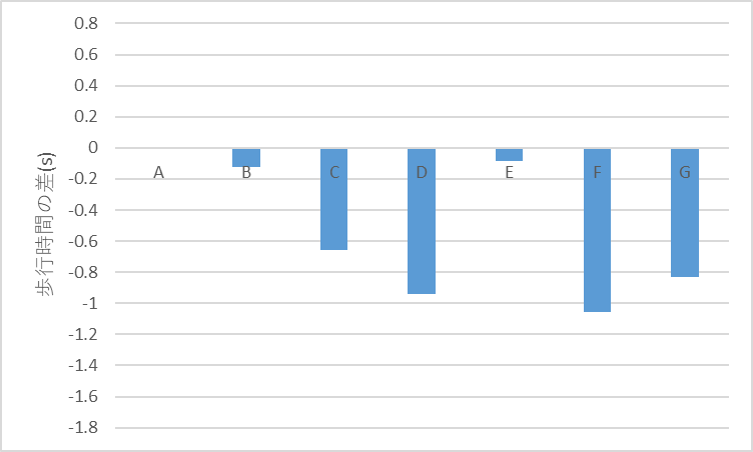
\includegraphics[width=0.8\linewidth]{fig/後速度早5YR天然.png}
    }
    \caption{システム未使用時とバーチャル床が後ろから追い越してくるシステム使用時のゴールまでの時間差(5YR天然)}
    \label{fig:5YRten}
\end{figure}

\begin{figure}[H]
    \centering
    \fbox{
        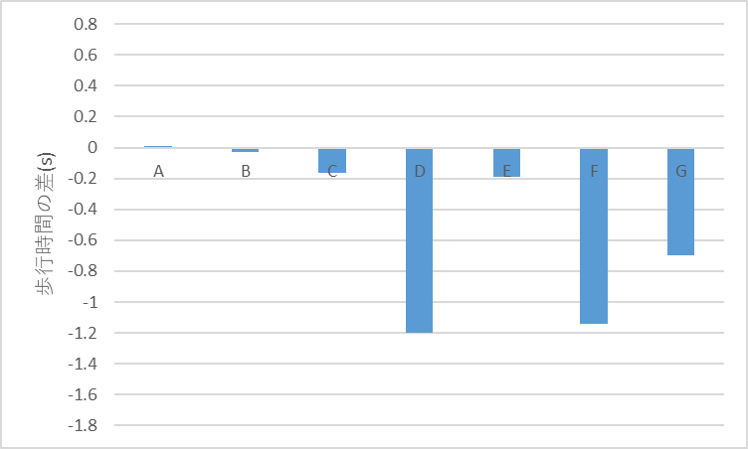
\includegraphics[width=0.8\linewidth]{fig/後速度早5RP天然.png}
    }
    \caption{システム未使用時とバーチャル床が後ろから追い越してくるシステム使用時のゴールまでの時間差(5RP天然)}
    \label{fig:5RPten}
\end{figure}

\begin{figure}[H]
    \centering
    \fbox{
        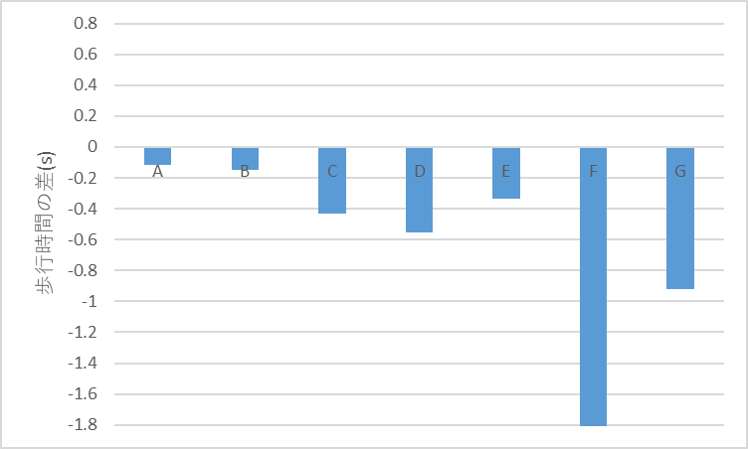
\includegraphics[width=0.8\linewidth]{fig/後速度早5RP人工.png}
    }
    \caption{システム未使用時とバーチャル床が後ろから追い越してくるシステム使用時のゴールまでの時間差(5RP人工)}
    \label{fig:5RPjinko}
\end{figure}


\section{考察}
今回仮説としてユーザの行動制御ができると考えていたリアルテクスチャは,効果が無かったことから,
ユーザに対してバーチャル床が見えやすい状態では実際の床にテクスチャを近似させる効果はないことが考察できた.
しかし,「砂利が一番好き.現実空間の床を消せてる.」や「砂利が模様が一番わかりやすかった」というコメントから実際の床にテクスチャを近似させるよりも
動いていることが分かりやすいテクスチャを作るほうが重要だと考察できる.


バーチャル床が後ろからユーザを追い越す動きをした場合,5YR人工は遅い速度感を与えることはできたが他のテクスチャは何も与えられなかった.
しかし,5YR天然,5RP人工,そして一番最も本物の床に見られていた5RP天然は定量評価の結果,システム未使用時に比べ,歩行時間が短くなっていた.
これらは共通して実際の床の色と色相環で見て,反対に位置する色が多い.
このことから色は現実の床と近似させないことで効果が強まると考えられる.
また,このバーチャル床の動かし方は上記の結果から
速度感を低下させ,ユーザの歩行速度を上昇させる効果があると考察できる.


バーチャル床が前から迫ってくる場合,遅い速度感を与えることはできなかったが,5YR天然は速い速度感を与えることには成功した.
さらに,定量評価の結果から,5YR人工とリアルテクスチャである5G人工は半数以上の被験者が歩行速度が低下していた.
これにより,床と同じ模様バーチャル床を前から迫ってくる動かし方は速度感を上昇させ,ユーザの歩行速度を遅くさせることが示唆された.
5G天然と5B砂利は体感歩行距離を長くしていたことから,テクスチャによってはこのバーチャル床の動き方は距離感に影響を与えることが示唆された.


これらの結果から,中間地点では歩行時間のプラスマイナスは分かれていたにもかかわらず,ゴール地点では
歩行時間が短くなっていたことから,本システムは一定時間経過後に効果が出始めることが考えられる.
しかし,今回の実験では効果が衰退し始めるタイミングはわからなかった.
今回のシステムはシースルー型のHMDを使用したため,ビデオスルー型のHMDを使用した場合ではバーチャル床の見え方が変わることが想定できるため
効果が変わってくることも考えられた.
